\chapter{仿真与差分测试框架}

\section{框架介绍}

为了提高处理器开发效率,我们自己开发了仿真与差分测试框架,分为SoC-Simulator与CEMU(CQU Emulator)两个部分。

\section{SoC-Simualtor}

SoC-Simulator是我们开发的一个基于Verilator的SoC仿真框架。它使用C++语言编写,通过软件实现了AXI Slave设备功能。其内置了MMIO Crossbar、UARTLite、UART8250、NSCSCC confreg等设备,能够满足运行龙芯杯功能测试、性能测试、系统测试,启动u-boot、uCore和Linux的需求。

此外,SoC-Simulator还能够支持AXI延迟的自定义,在我们开发处理器期间经过了多次测试,在AXI延迟设置为23周期的情况下,SoC-Simulator仿真的性能得分与上板真实成绩误差在1分以内。

同时得益于Verilator的仿真效率,以我们的CPU核\cpuname 为例,在当前主流的台式机(AMD Ryzen 7 5800X)上实现了高速测试,2秒完成功能测试(含Trace比对),7秒钟完成性能测试并输出CP0 count寄存器的结果。同时,在SoC-Simulator上运行uCore可以10秒内进入shell,运行Linux v5.19配合我们基于defconfig修改的配置大约4分钟开始执行init进程,相比于改一行RTL综合上板10分钟以上的时间,这大大方便了我们修改RTL后及时得到IPC反馈与问题定位与调试工作。

\begin{figure}[h]
    \centering
    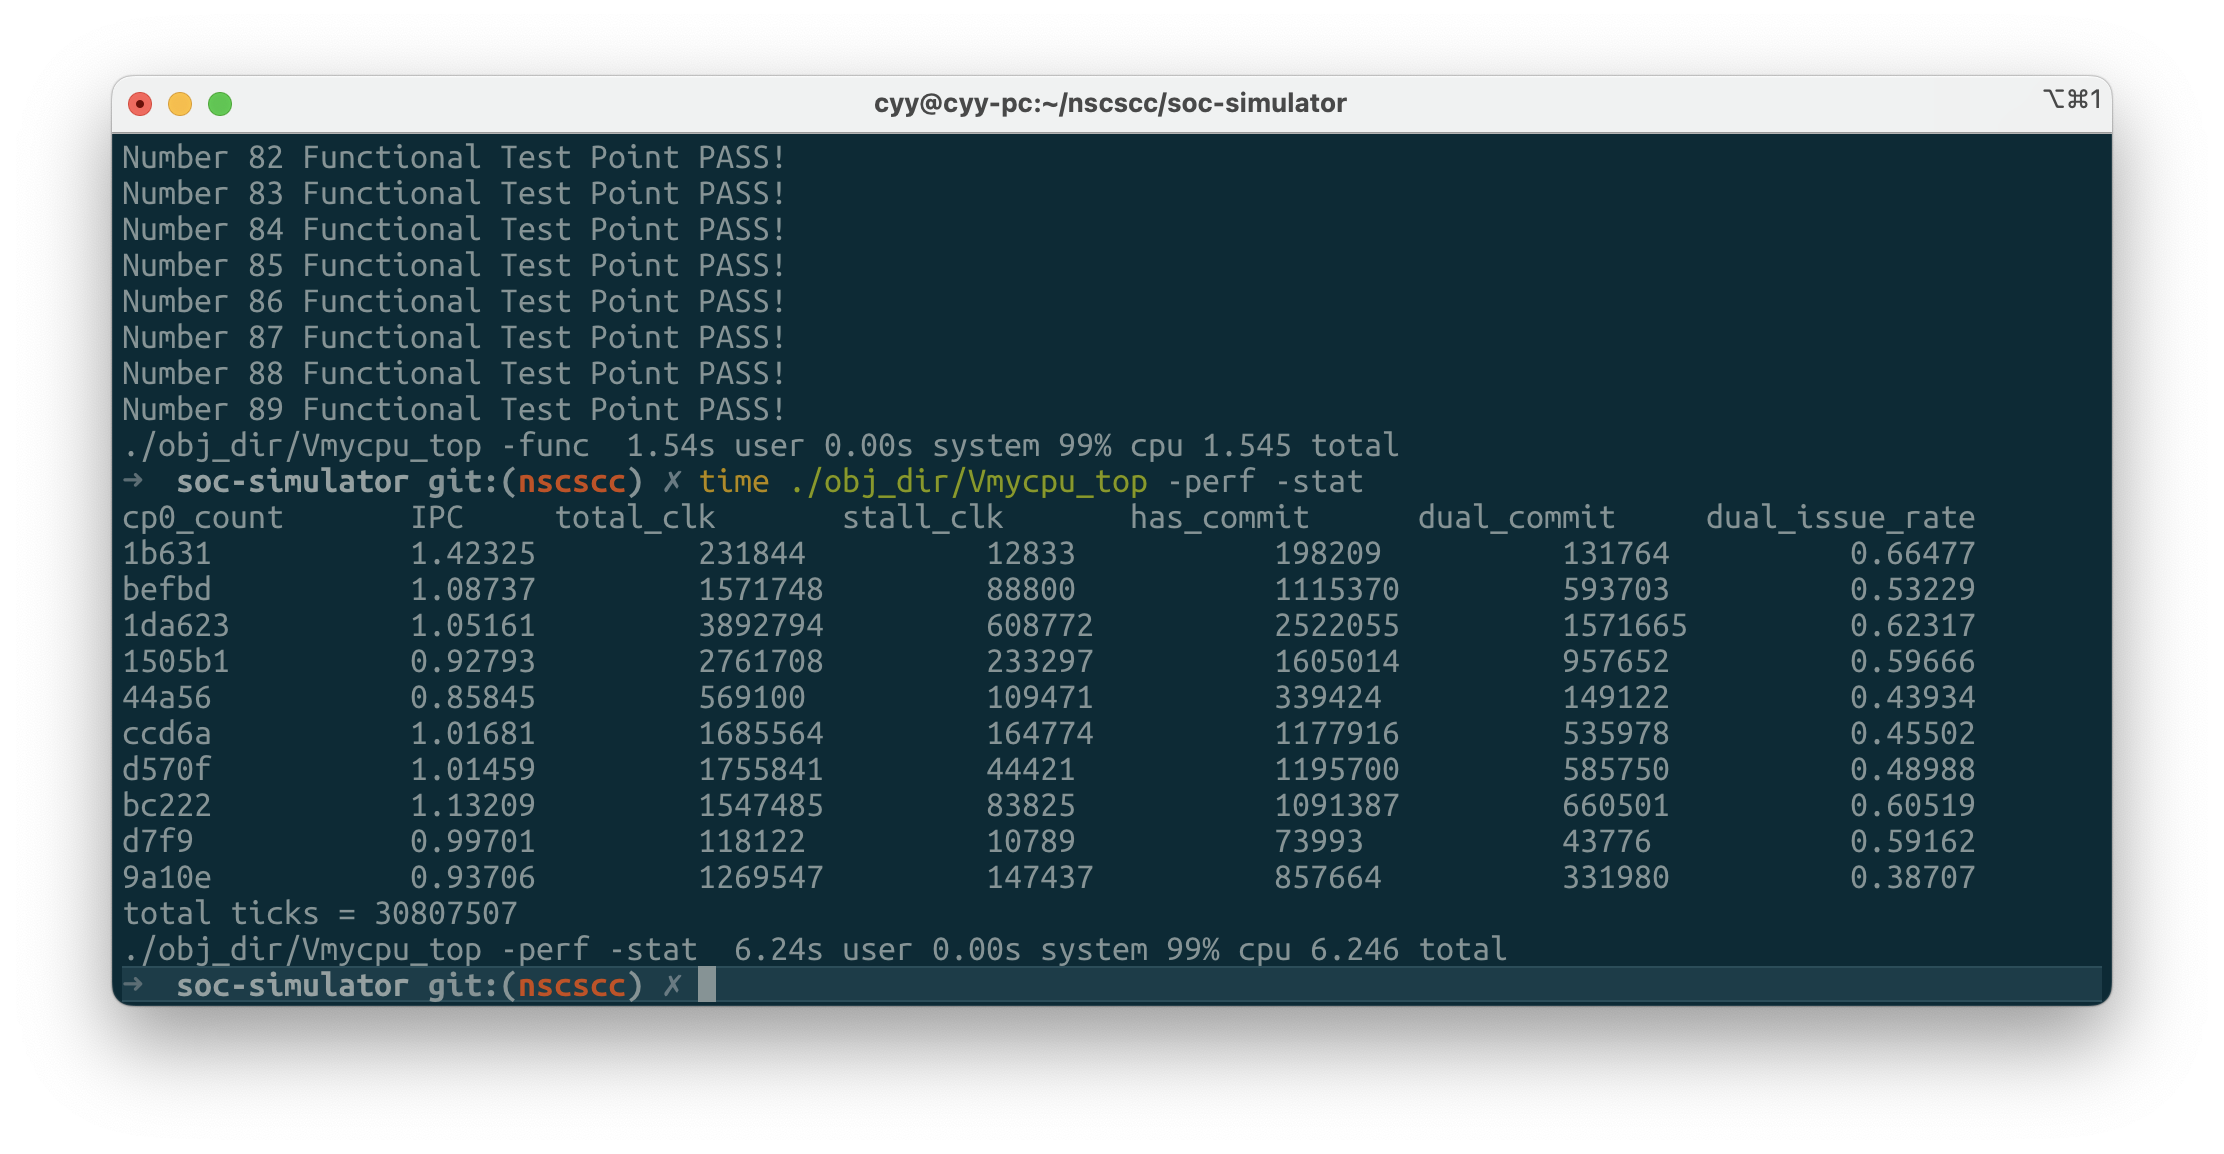
\includegraphics[width=\linewidth]{soc_simulator_func_perf.png}
    \caption{SoC-Simulator运行功能测试与性能测试}
\end{figure}

\begin{figure}[h]
    \centering
    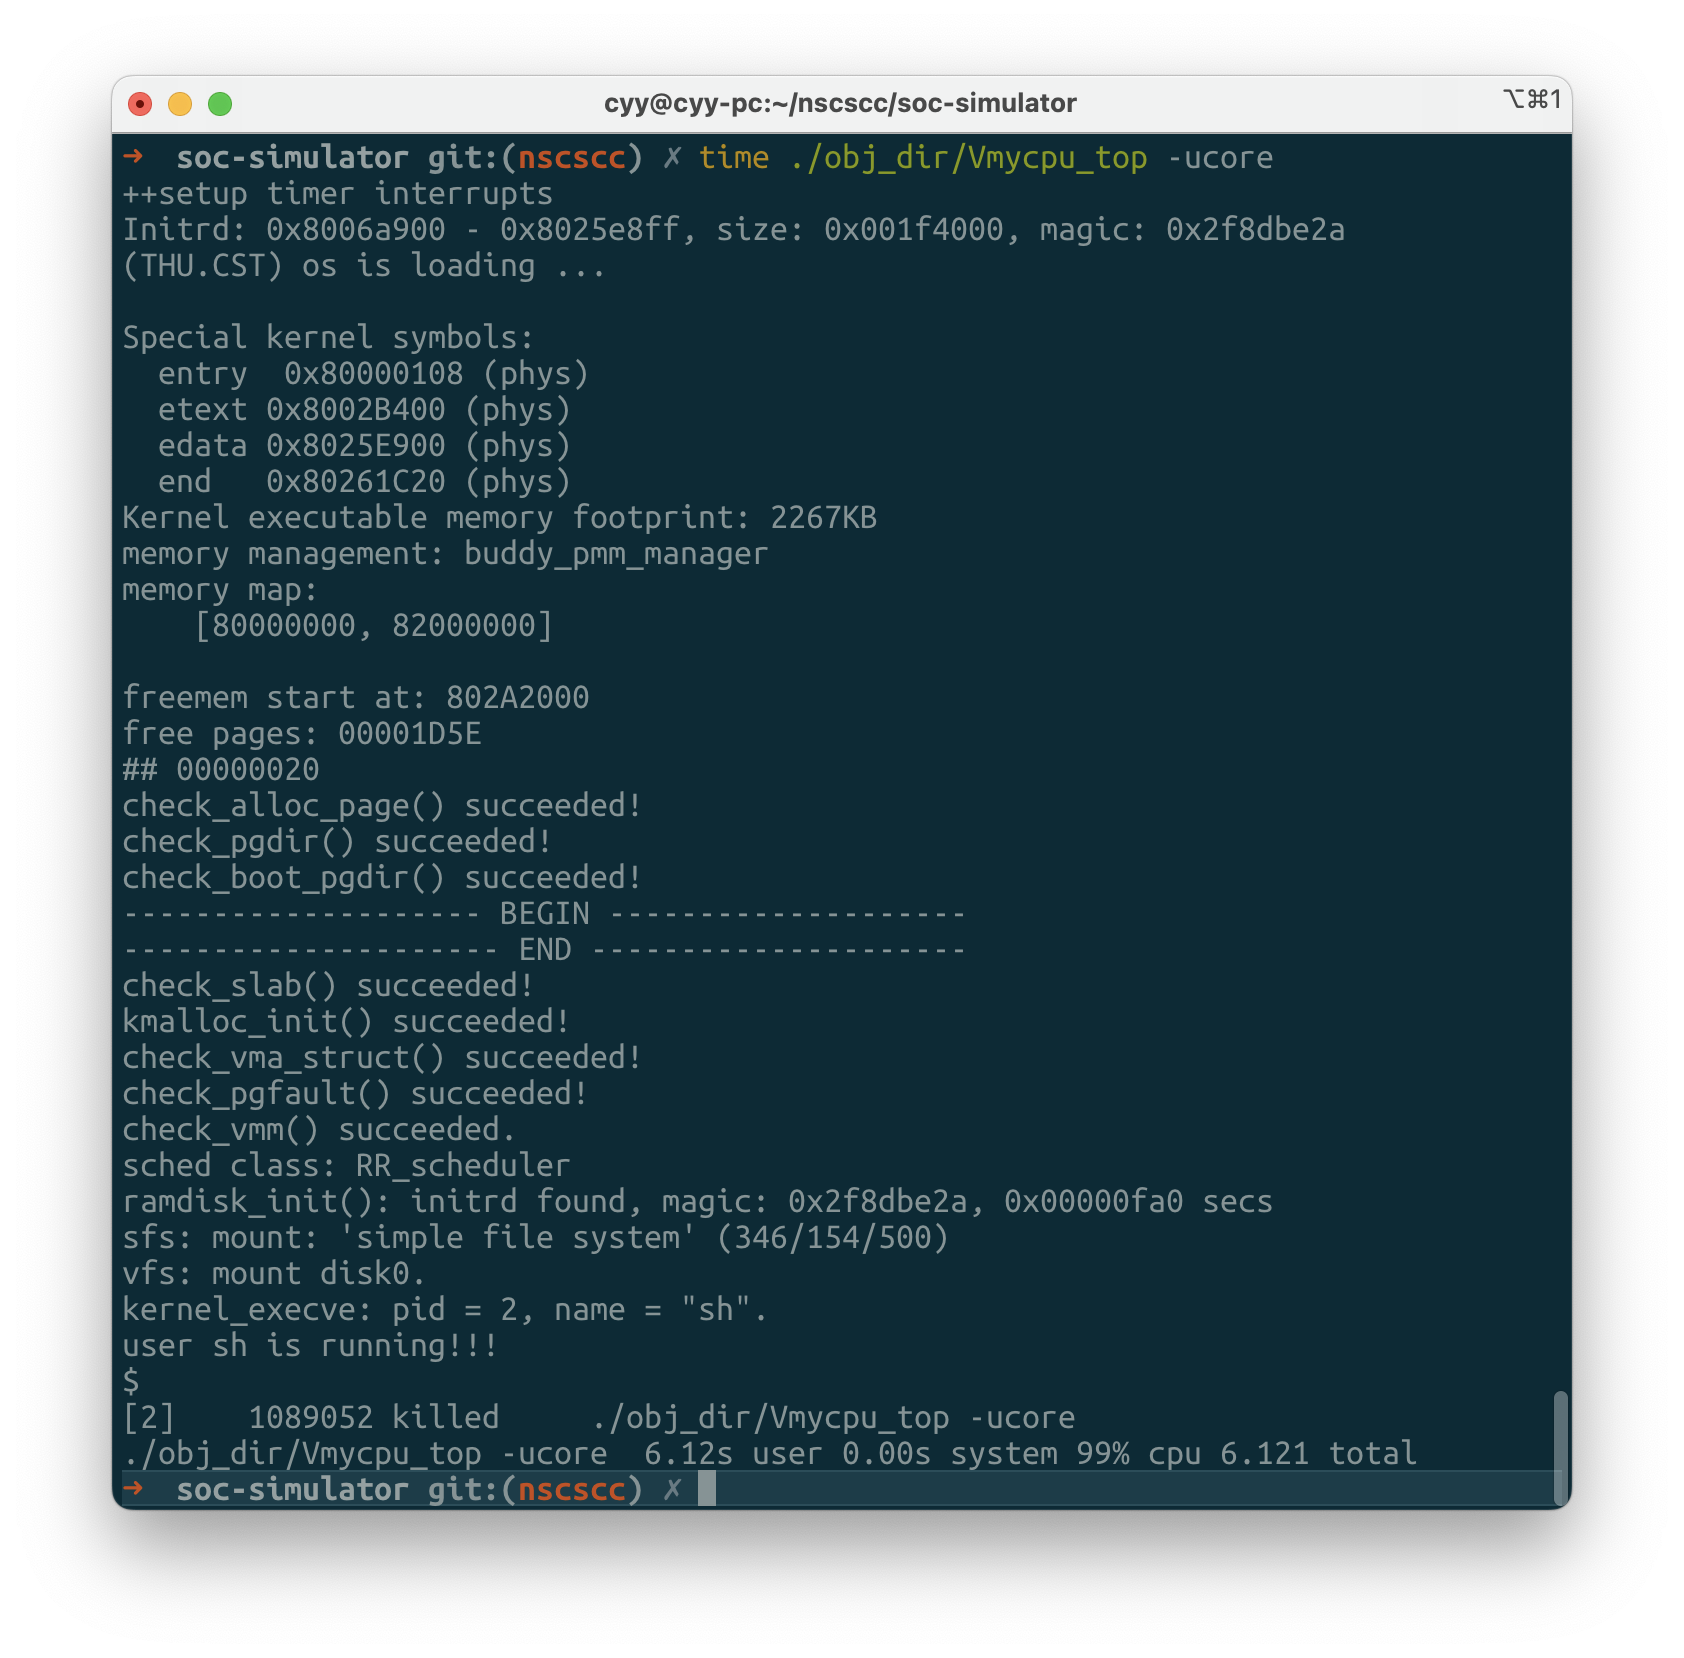
\includegraphics[width=\linewidth]{soc_simulator_ucore.png}
    \caption{SoC-Simulator运行uCore}
\end{figure}

\begin{figure}[h]
    \centering
    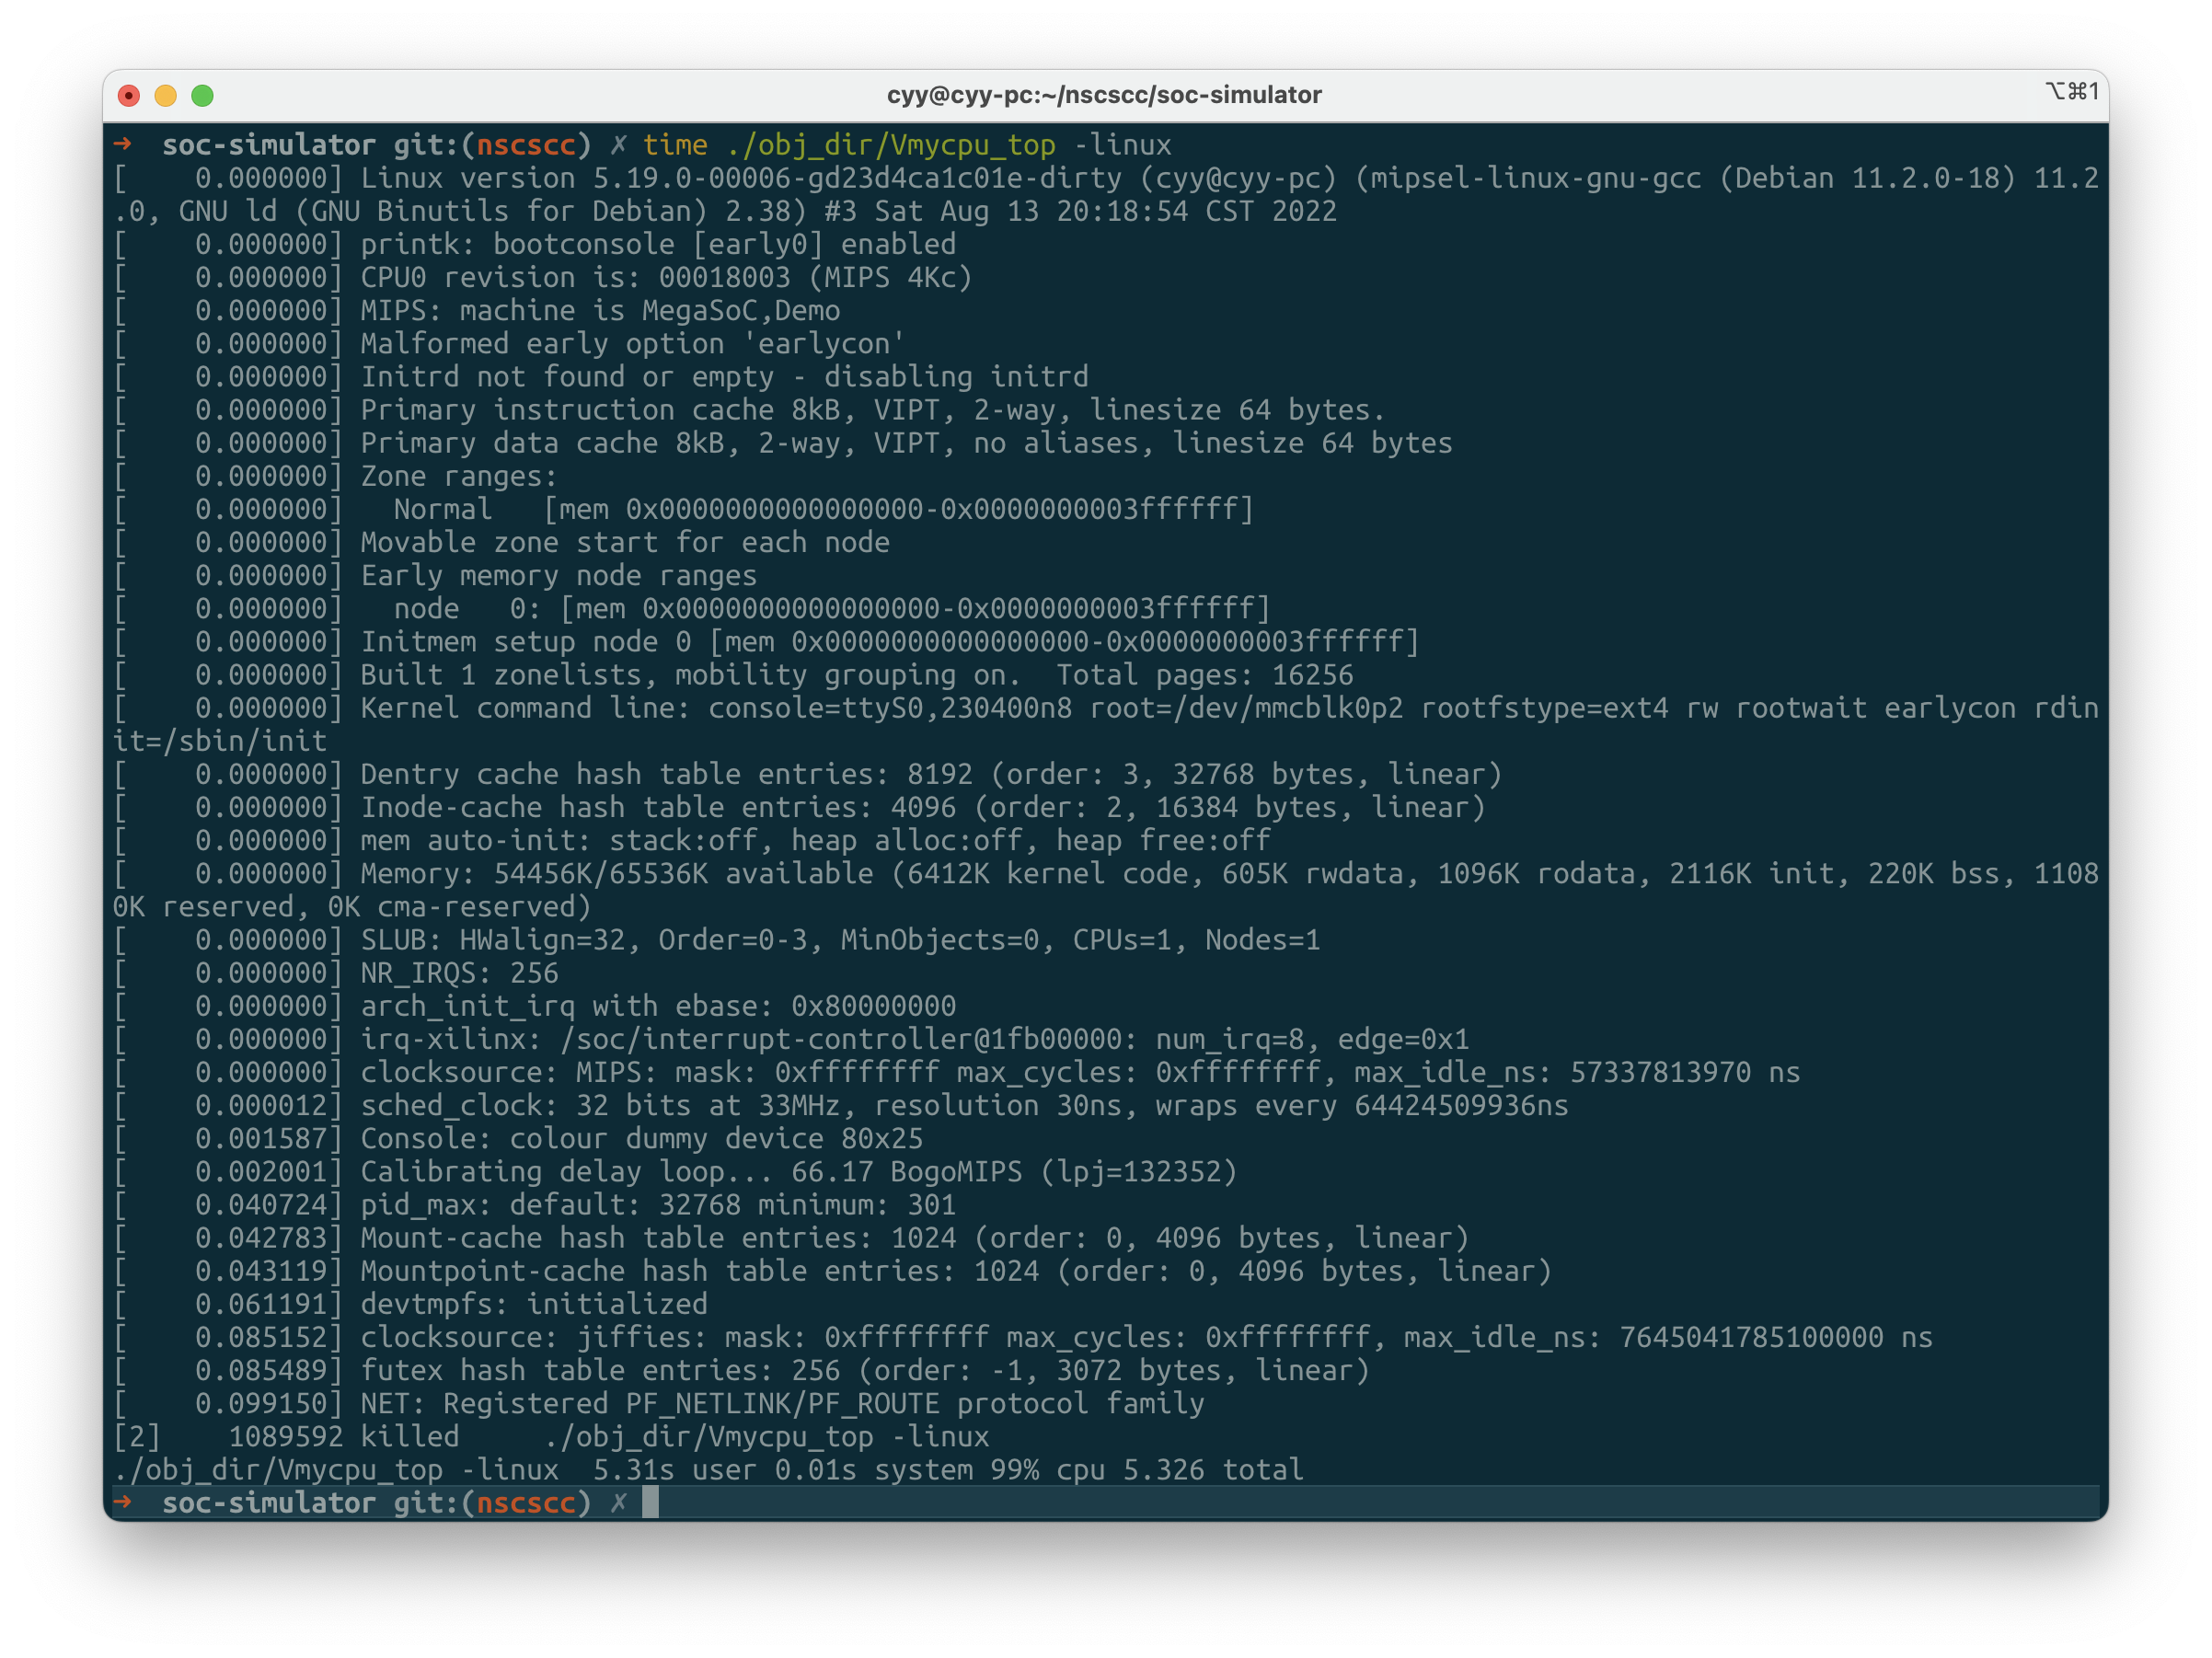
\includegraphics[width=\linewidth]{soc_simulator_linux.png}
    \caption{SoC-Simulator运行Linux}
\end{figure}

\section{CEMU}

CEMU(CQU Emulator)是我们开发的一个CPU模拟器,目前支持了RV64IMA与MIPS Release 1指令集,LoongArch32的支持正在实现中,我们使用它与\cpuname 进行差分测试,

由于CEMU与SoC-Simulator都是我们自行开发的,因而采用了完全相同的外设接口(C++的抽象类),从而CEMU与SoC-Simulator能够运行在完全相同的SoC环境中,并通过处理器RTL输出的CP0 Count、CP0 Cause、CP0 Random、是否中断等信号对CEMU的各寄存器状态进行同步,这帮助我们在\cpuname 调通uCore后仅2天时间就完成了Linux的调试。

在\cpuname 调试过程中,我们也不断完善了CEMU与SoC-Simulator的difftest功能。例如添加了内存写回时AXI传入数据与CEMU内存的对比功能,以及条件输出波形图等功能(避免调试Linux时波形图输出消耗大量存储资源)。并在调试Linux期间为了调试Linux Kernel自身写入的指令(如EBASE段的异常处理,这部分不在vmlinux的反汇编中)的执行过程,在差分测试错误时能够将CEMU的整个内存转储出来,再通过objdump反汇编即可知道动态写入的指令,便于通过指令序列观察处理器执行可能存在的问题(例如常见的延迟槽出现先前测试未覆盖的指令)。

\begin{figure}[h]
    \centering
    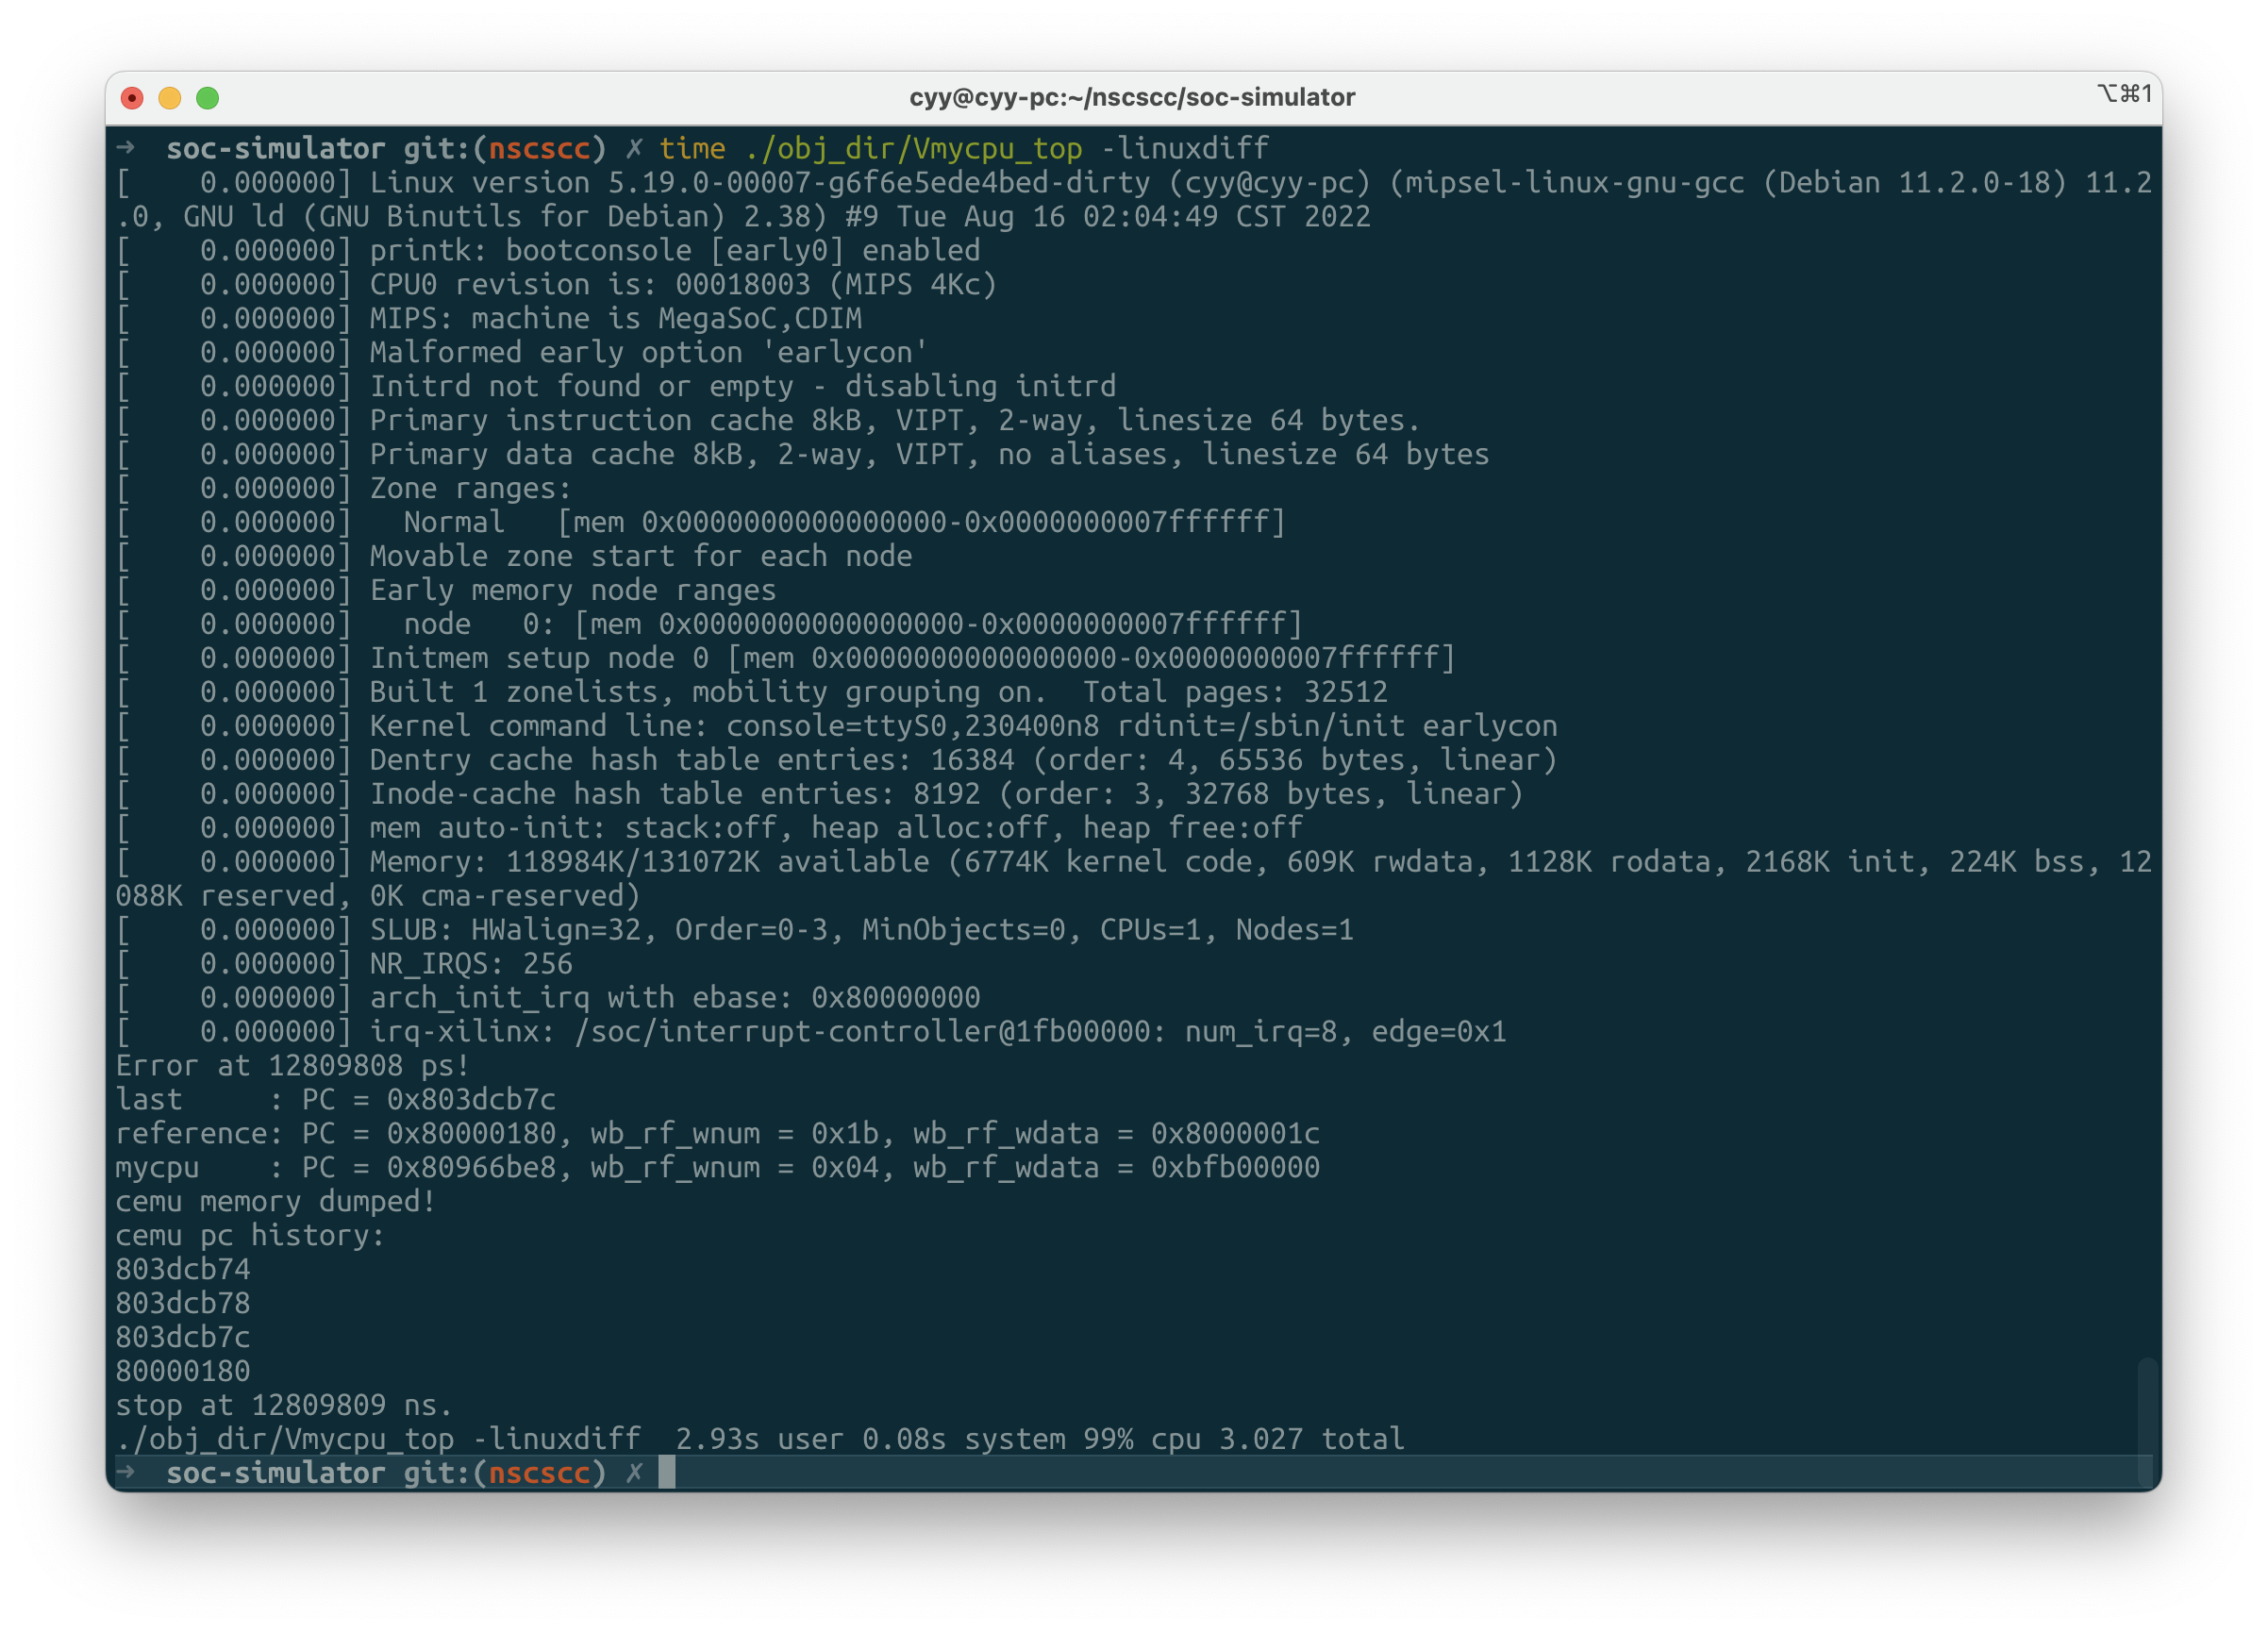
\includegraphics[width=\linewidth]{soc_simulator_linuxdiff.png}
    \caption{SoC-Simulator与CEMU差分测试错误提示}
\end{figure}